%% Figures
% \renewcommand{\thesubfloat}{Panel \Alph{subfloat}:}
\setcounter{figure}{0}

\clearpage
\newpage
\begin{figure}[ht!]
\centering
\caption{Deposits and Loans in Decentralized Financial Lending Markets}\label{fig:defi}
\caption*{This figure presents the total deposits (Panel A) and loans (Panel B) in US dollars within the DeFi lending sector from 2018 to 2023. The data is from DefiLlama. }
\subfloat[Total Deposit Amount in USD]{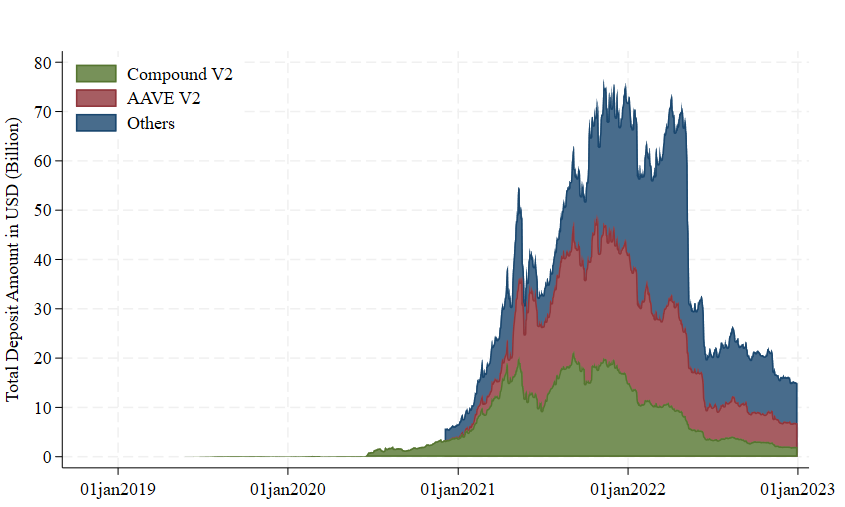
\includegraphics[width=0.95\linewidth]{figure/Deposit.png}}


\subfloat[Total Loan Amount in USD]{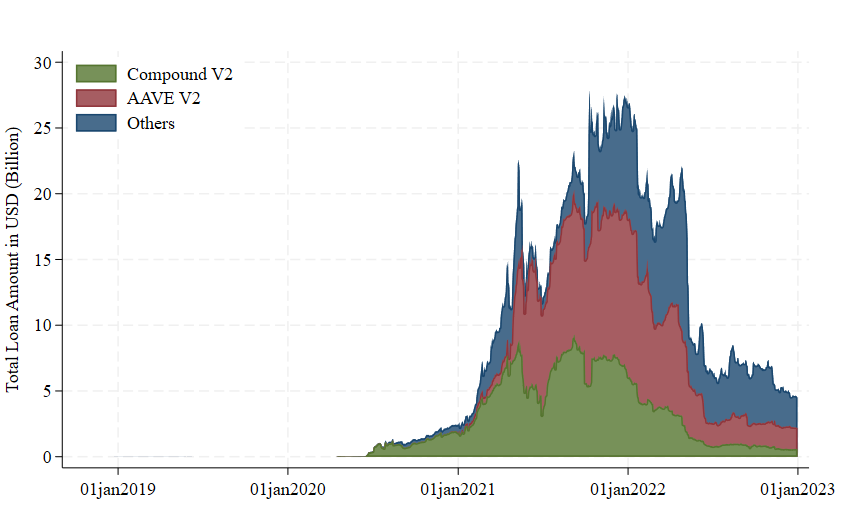
\includegraphics[width=0.95\linewidth]{figure/Loan.png}}

\end{figure}

\clearpage
\newpage
\begin{figure}[ht!]
\centering
\caption{Mechanisms of a Decentralized Financial Lending Platform}\label{fig:mechanism}
\caption*{This figure presents how AAVE facilitates borrowing and lending. The mechanisms are similar to those of Compound. Panel A provides an example of borrowing and lending, and Panel B presents positions after liquidation. }
\bigskip
\subfloat[Borrowing and Lending]{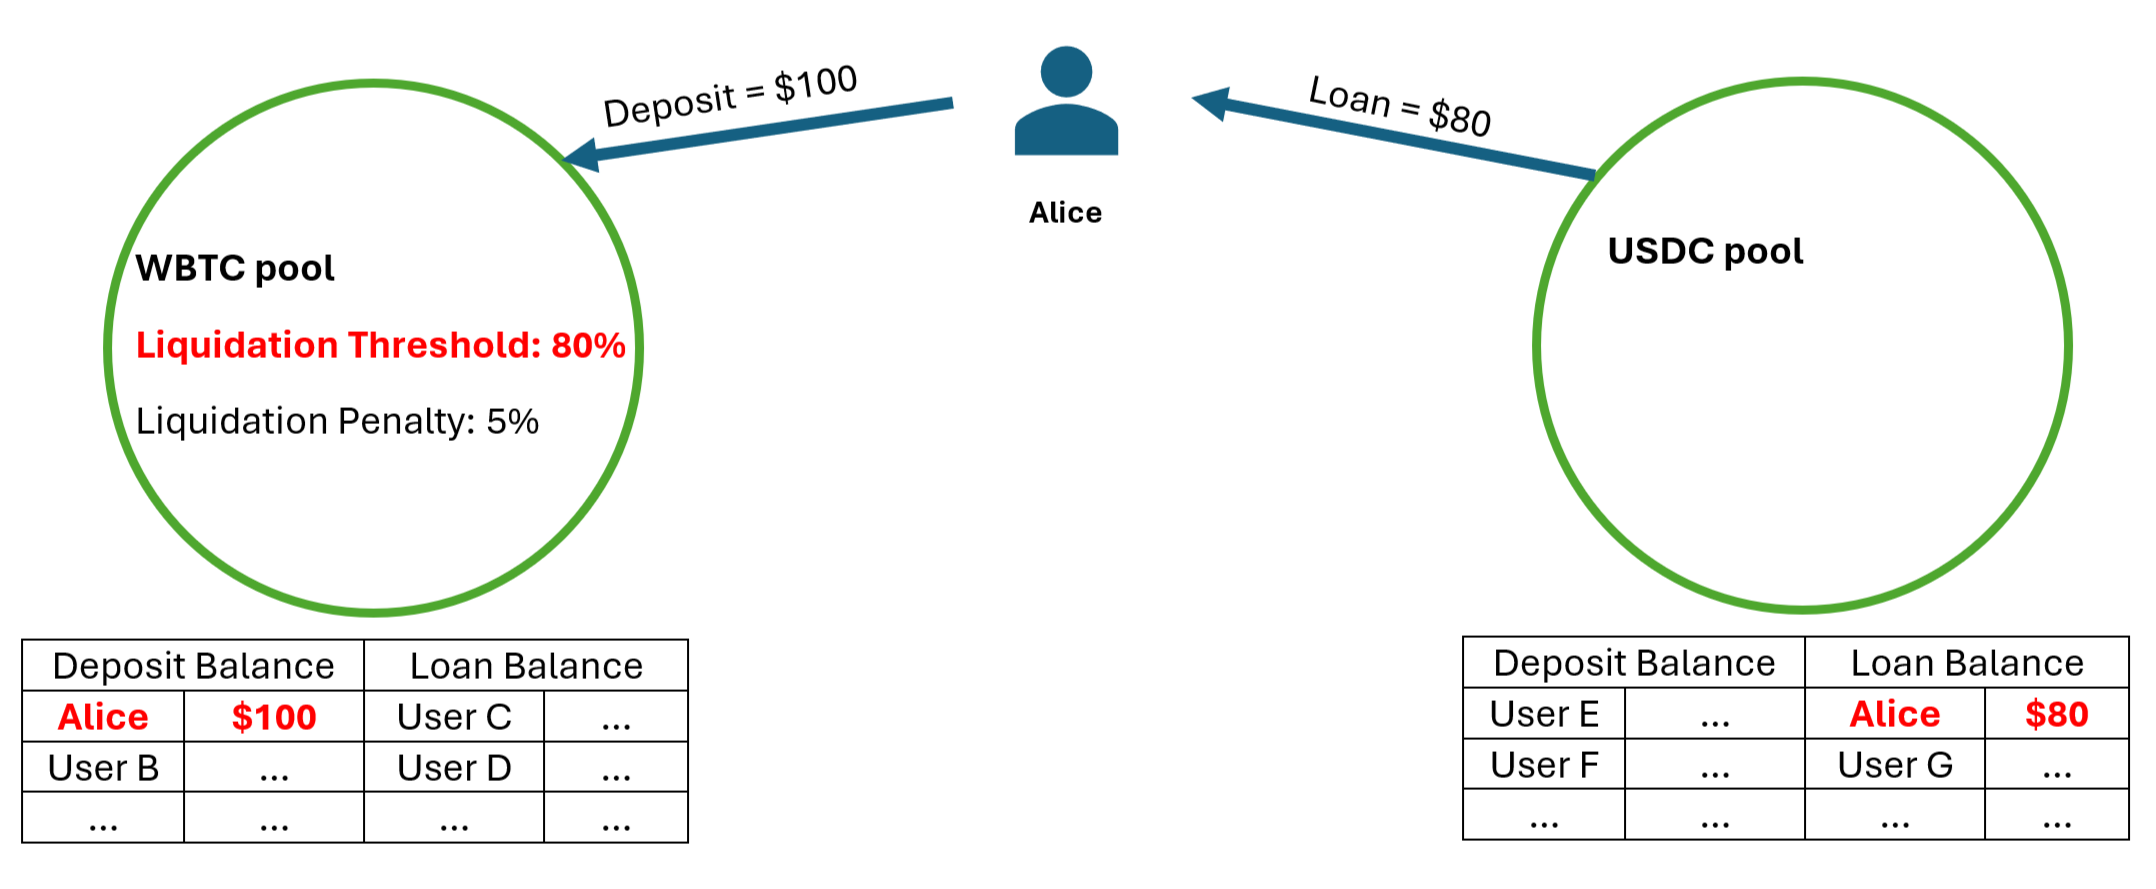
\includegraphics[width=\linewidth]{figure/mechanism1.png}}

\bigskip
\subfloat[Positions after Liquidation]{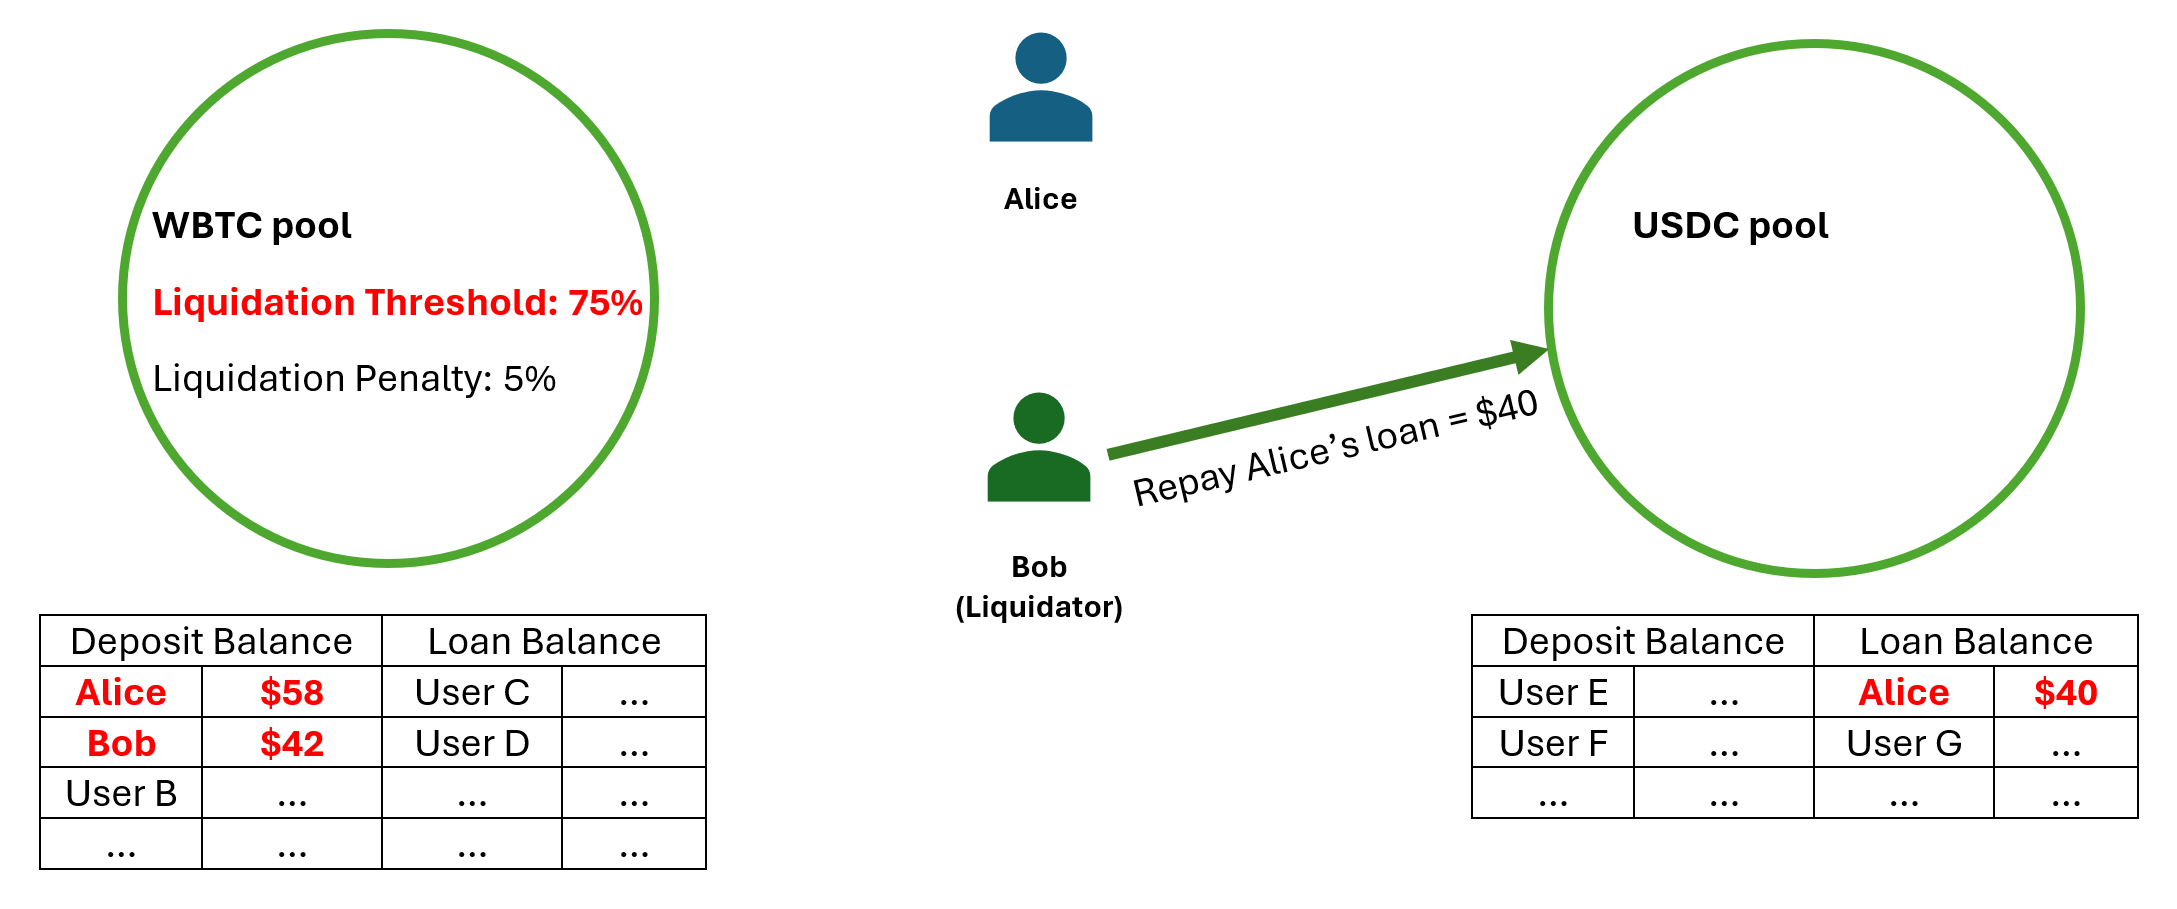
\includegraphics[width=\linewidth]{figure/mechanism2.png}}

\end{figure}

\clearpage
\newpage

\begin{figure}[ht!]
\centering
\caption{Governance Process}\label{fig:governance}
\caption*{This figure outlines the governance process within DeFi lending platforms. After creation, a proposal enters a discussion stage, allowing the community to evaluate its efficiency in a public forum. Following the discussion, the proposal advances to a voting stage. A successful proposal must obtain a majority of affirmative votes and exceed a predefined quorum number. If the proposal fails to meet these requirements, it will be rejected. The successful proposal then enters a timelock period, typically lasting one to two days, before execution. }
\subfloat{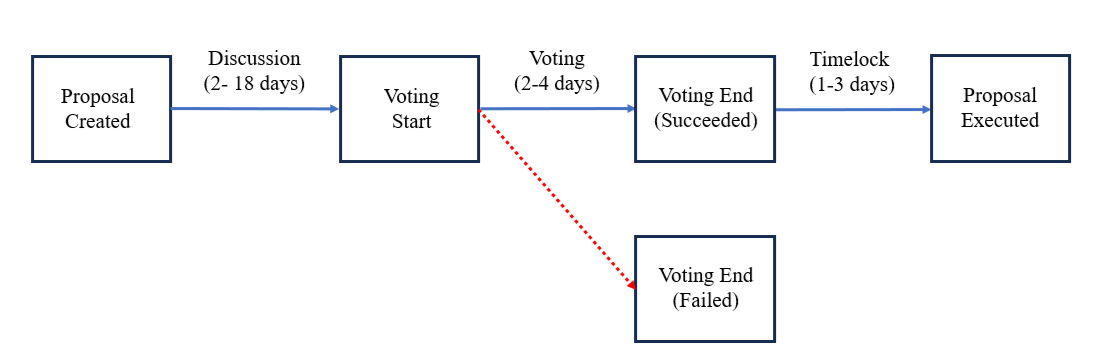
\includegraphics[width=\linewidth]{figure/voting.png}}

\end{figure}

\clearpage
\newpage


\begin{landscape}
\begin{figure}[ht!]
\centering
\caption{Deposits and Loans by Pools}\label{fig:deposit_loan_bypool}
\caption*{This figure plots the total deposit and loan amounts in US dollars of lending pools of USDC, DAI, WBTC, and WETH and other pools on AAVE and Compound from January 2021 to January 2023. The total deposit or total loan of all other pools is calculated by summing up the number of individual ones. }

\centering
\subfloat[Total Deposit Amount in USD on AAVE]{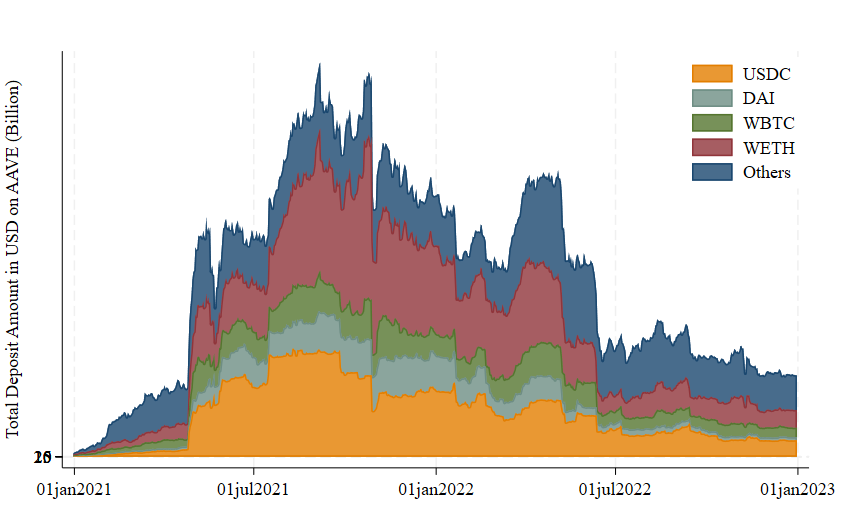
\includegraphics[width=0.48\linewidth]{figure/Deposit_AAVE_bypool.png}}
\subfloat[Total Loan Amount in USD on AAVE]{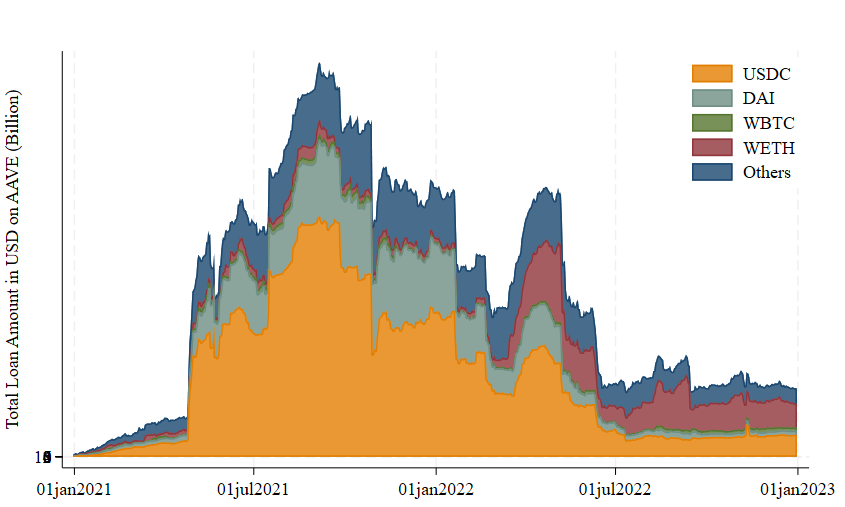
\includegraphics[width=0.48\linewidth]{figure/Loan_AAVE_bypool.png}}

\subfloat[Total Deposit Amount in USD on Compound]{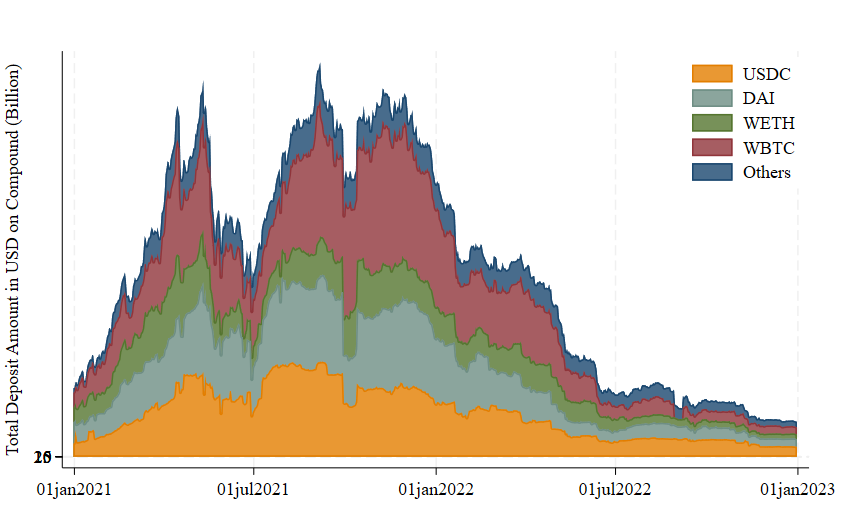
\includegraphics[width=0.48\linewidth]{figure/Deposit_COMP_bypool.png}}
\subfloat[Total Loan Amount in USD on Compound]{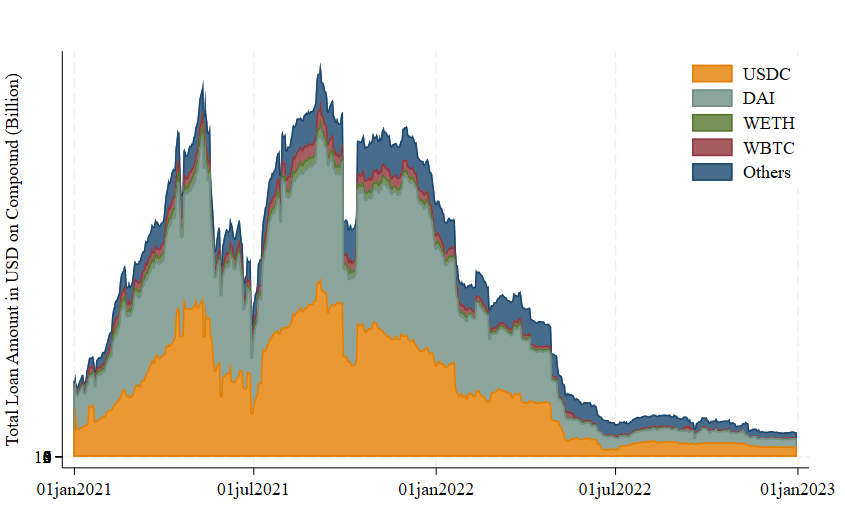
\includegraphics[width=0.48\linewidth]{figure/Loan_COMP_bypool.png}}

\end{figure}

\end{landscape}


\clearpage
\newpage


\begin{landscape}
\begin{figure}[ht!]
\centering
\caption{ Borrowing Rates}\label{fig:borrowingrate_major}
\caption*{This figure plots the borrowing rate of lending pools of USDC, DAI, WBTC, and WETH on AAVE and Compound and the Secured Overnight Financing Rate from January 2021 to January 2023.  }

\centering
\subfloat[USD Coin (USDC)]{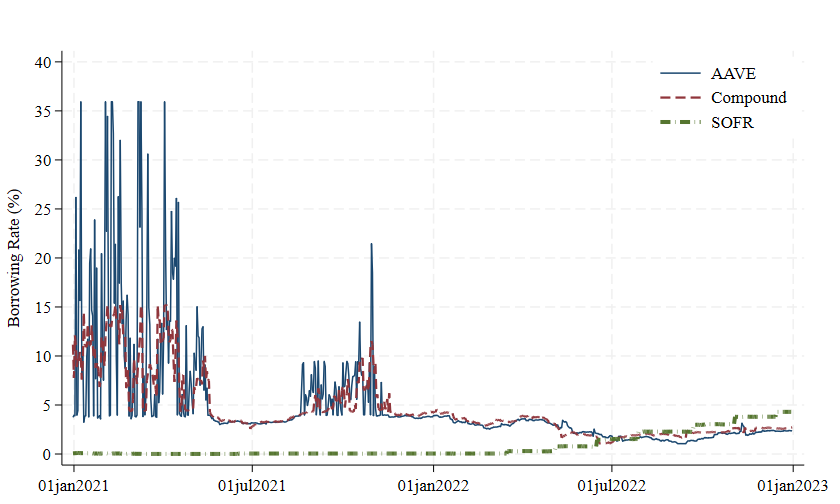
\includegraphics[width=0.48\linewidth]{figure/USDC_BRate.png}}
\subfloat[Dai (DAI)]{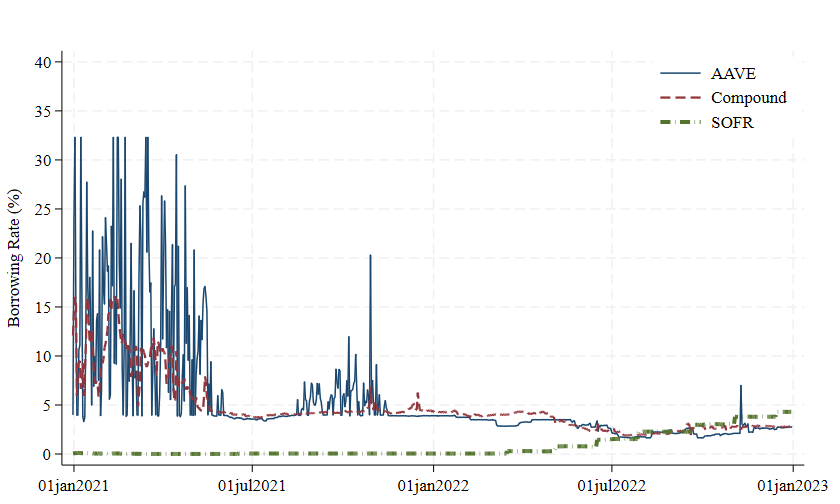
\includegraphics[width=0.48\linewidth]{figure/DAI_BRate.png}}

\subfloat[Wrapped Bitcoin (WBTC)]{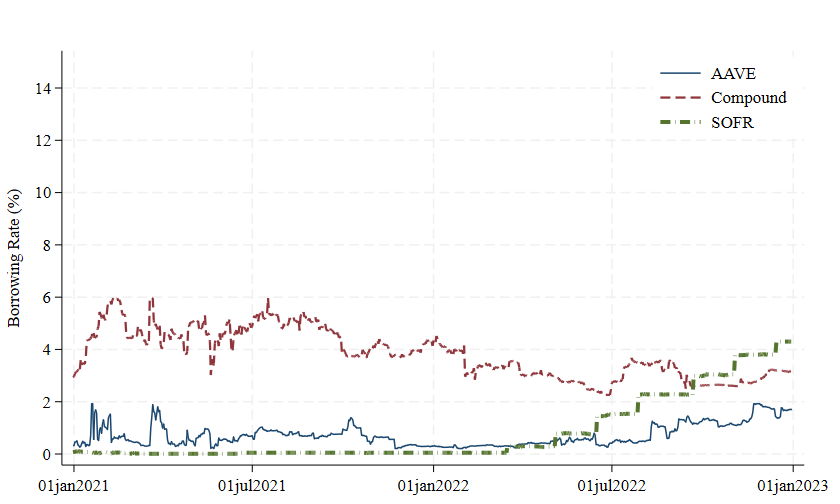
\includegraphics[width=0.48\linewidth]{figure/WBTC_BRate.png}}
\subfloat[Wrapped Ethereum (WETH)]{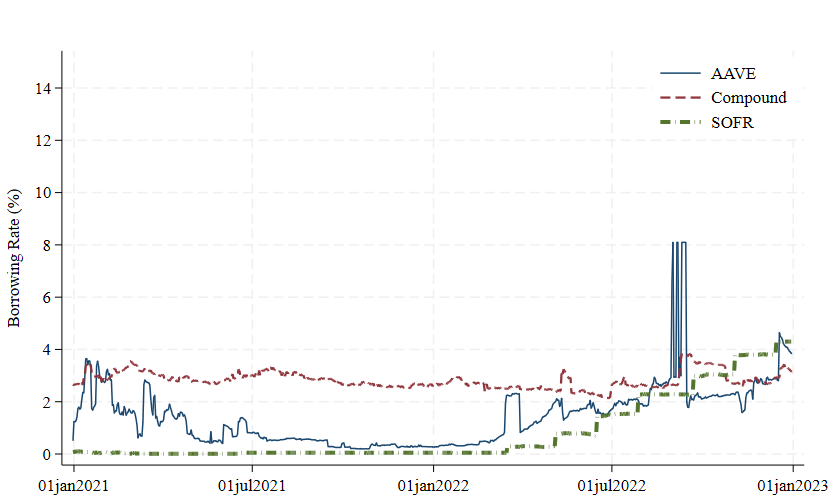
\includegraphics[width=0.48\linewidth]{figure/WETH_BRate.png}}

\end{figure}

\end{landscape}

\clearpage
\newpage
% \begin{landscape}
\begin{figure}[ht!]
\centering
\caption{Dynamics of Loan Balances}\label{fig:dynamics_borrow}
\caption*{This figure plots the estimations of $\beta$ coefficients from the Poisson pseudo-maximum likelihood regression: $TotalBorrow_{i,t}^p=\sum_{j=-7}^{7}\beta_jTreated_{i}^p\times I_j+\delta Treated_{i}^p+\sum_{s=-7}^{7}\sigma_sI_s+\textit{Borrower FE} + \textit{Collateral}\times\textit{Week FE}+\epsilon_{i,t}^p$, where $TotalBorrow_{i,t}^{p}$ represents the total loan balance in account $i$ on platform $p$ at the end of week $t$. $Treated_{i}^{p}$ is a binary variable that takes a value of 1 if account $i$ experiences a relaxation in margin requirements. $I_j$ is an indicator variable for weeks relative to the week of proposal execution. Standard errors are clustered at the borrower and week levels. The bars surrounding each coefficient represent the 5\% and 95\% confidence intervals.  }

\bigskip

% \subfloat[TotalBorrow (Dollar)]{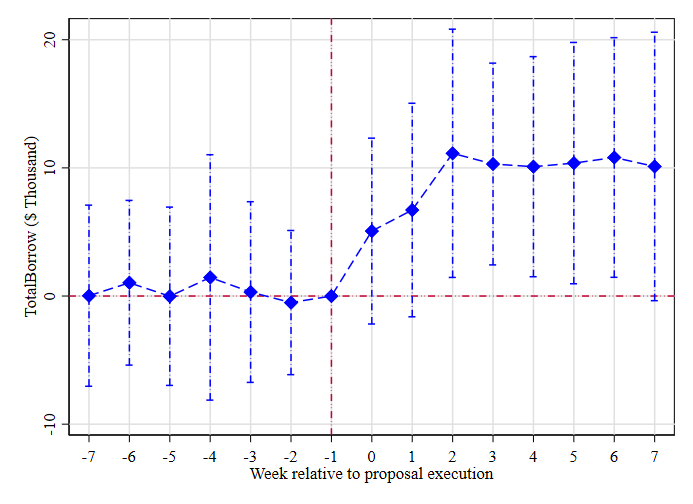
\includegraphics[width=0.45\linewidth]{figure/borrow_dollar.png}}
\subfloat{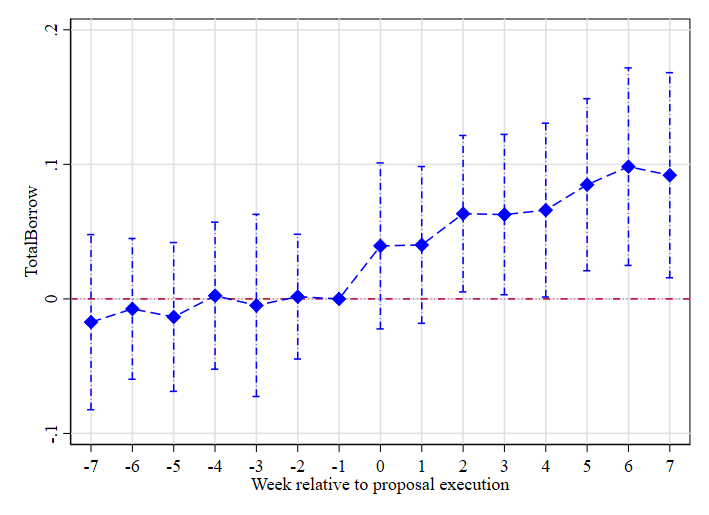
\includegraphics[width=\linewidth]{figure/borrow_pp.png}}
\end{figure}
% \end{landscape}

\clearpage
\newpage



% \begin{landscape}
\begin{figure}[ht!]
\centering
\caption{Dynamics of Deposit Balances}\label{fig:dynamics_deposit}
\caption*{This figure plots the estimations of $\beta$ coefficients from the Poisson pseudo-maximum likelihood regression: $Deposit_{i,t}^{c,p}=\sum_{j=-7}^{7}\beta_jTreated_{i}^p\times I_j+\delta Treated_{i}^p+\sum_{s=-7}^{7}\sigma_sI_s+\textit{Borrower FE} + \textit{Collateral}\times\textit{Week FE}+\epsilon_{i,t}^p$, where $Deposit_{i,t}^{c,p}$ represents the US dollar amount of the deposit balance in the treated or control pool of cryptocurrency $c$ on platform $p$ held by account $i$ at the end of week $t$. $Treated_{i}^{p}$ is a binary variable that takes a value of 1 if account $i$ experiences a relaxation in margin requirements. $I_j$ is an indicator variable for weeks relative to the week of proposal execution. Standard errors are clustered at the borrower and week levels. The bars surrounding each coefficient represent the 5\% and 95\% confidence intervals. }

\bigskip

% \subfloat[Deposit (Dollar)]{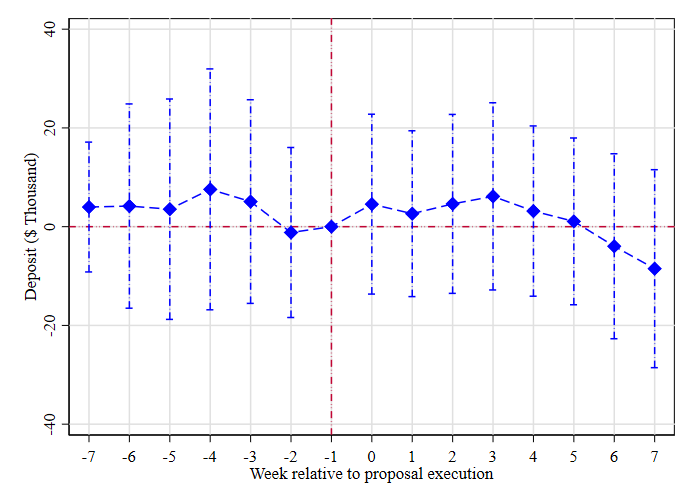
\includegraphics[width=0.45\linewidth]{figure/deposit_dollar.png}}
\subfloat{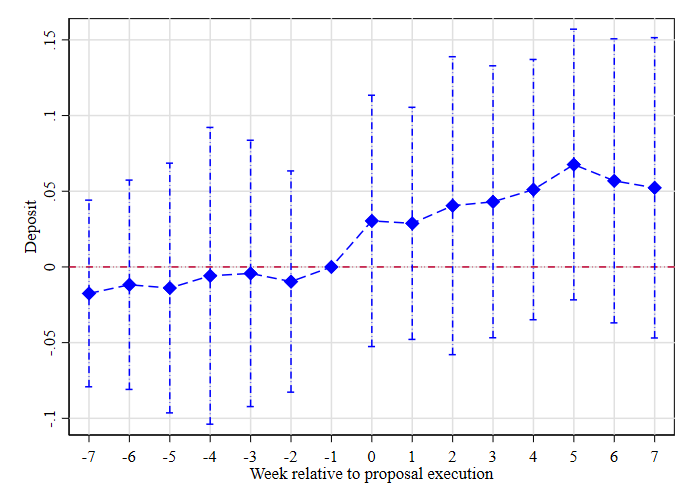
\includegraphics[width=\linewidth]{figure/deposit_pp.png}}

\end{figure}

% \end{landscape}

\clearpage
\newpage


\begin{landscape}
\begin{figure}[ht!]
\centering
\caption{Disproportionate Effects of Margin Requirements on Borrowers with Highly
Leveraged Positions}\label{fig:loandeposit_highlev}
\caption*{This figure repeats the analysis in Column (2) of Table \ref{tab:mainborrow} and Table \ref{tab:maindeposit} and plots the coefficient of $\beta_2$. Borrowers are sorted into quartiles based on the average leverage ratio, estimated using daily observations from the start of the event window to the day before the proposal discussion. Borrowers with the lowest leverage ratio are in the lowest quartile (Quartile 1). Borrowers with the highest leverage ratio are in the highest quartile (Quartile 4). The coefficient of $\beta_2$ for each quartile is presented. Standard errors are clustered at the borrower and week levels. The bars surrounding each coefficient represent the 5\% and 95\% confidence intervals. }

\bigskip

\subfloat[TotalBorrow]{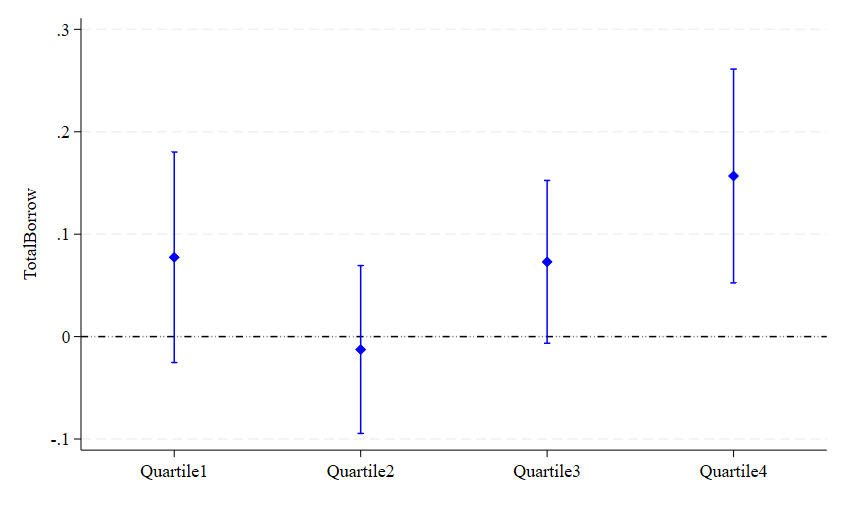
\includegraphics[width=0.45\linewidth]{figure/Heterogeneity/borrow.png}}
\subfloat[Deposit]{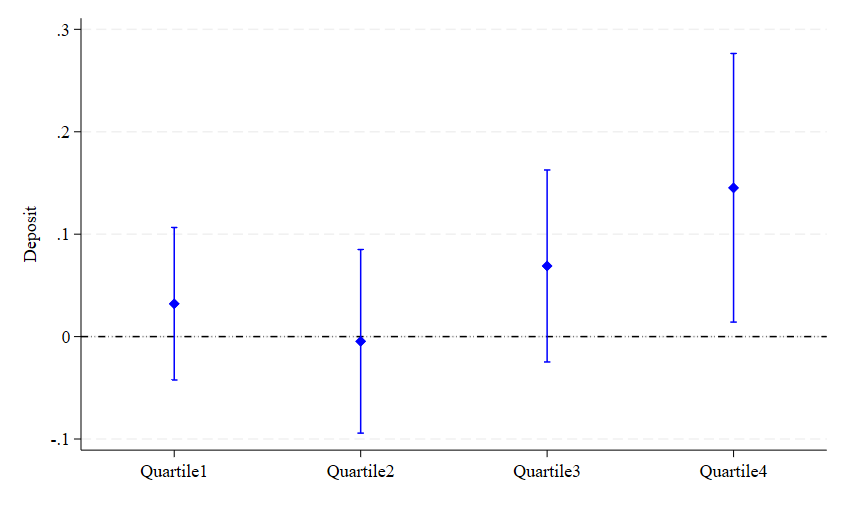
\includegraphics[width=0.45\linewidth]{figure/Heterogeneity/deposit.png}}
\end{figure}

\end{landscape}

\clearpage
\newpage


\begin{figure}[ht!]
\centering
\caption{Relaxed Margin Requirements and Leverage }\label{fig:post_lev}
\caption*{This figure repeats the same analysis in Column (2) of Table \ref{tab:mainborrow} and plots the coefficient of $\beta_2$. The dependent variable is $Leverage_{i,t}^p$, which represents the leverage of account $i$ on platform $p$ at the end of week $t$. The estimations are from the Ordinary Least Squares (OLS) regression model. Borrowers are sorted into quartiles based on the average leverage ratio, estimated using daily observations from the start of the event window to the day before the proposal discussion. Borrowers with the lowest leverage ratio are in the lowest quartile (Quartile 1). Borrowers with the highest leverage ratio are in the highest quartile (Quartile 4). The coefficient of $\beta_2$ for each quartile is presented. Standard errors are clustered at the borrower and week levels. The bars surrounding each coefficient represent the 5\% and 95\% confidence intervals. }

\subfloat{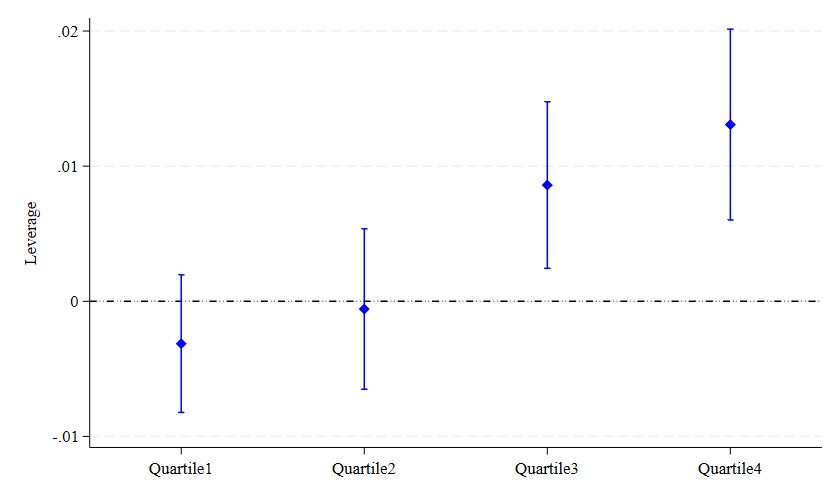
\includegraphics[width=\linewidth]{figure/Heterogeneity/lev.png}}
\end{figure}


\clearpage
\newpage


\begin{landscape}
\begin{figure}[ht!]
\centering
\caption{Dynamics of Leverage}\label{fig:dynamics_lev}
\caption*{This figure plots the estimations of $\beta$ coefficients from the Ordinary Least Squares regressions: $Leverage_{i,t}^{p}=\sum_{j=-7}^{7}\beta_jTreated_{i}^p\times I_j+\delta Treated_{i}^p+\sum_{s=-7}^{7}\sigma_sI_s+\textit{Borrower FE} + \textit{Collateral}\times\textit{Week FE}+\epsilon_{i,t}^p$, where $Leverage_{i,t}^{p}$ represents the leverage of account $i$ on platform $p$ at the end of week $t$. $Treated_{i}^{p}$ is a binary variable that takes a value of 1 if account $i$ experiences a relaxation in margin requirements. $I_j$ is an indicator variable for weeks relative to the week of proposal execution. Borrowers are sorted into quartiles based on the average leverage ratio, estimated using daily observations from the start of the event window to the day before the proposal discussion. Borrowers with the lowest leverage ratio are in the lowest quartile (Quartile 1). Borrowers with the highest leverage ratio are in the highest quartile (Quartile 4). Standard errors are clustered at the borrower and week levels. The bars surrounding each coefficient represent the 5\% and 95\% confidence intervals. }
\end{figure}

\end{landscape}

\clearpage
\newpage
\begin{landscape}
\begin{figure}[ht!]
\centering
\caption*{ Figure \ref{fig:dynamics_lev} - Continued from the previous page}
\subfloat[Quartile 1 (Lowest Leverage)]{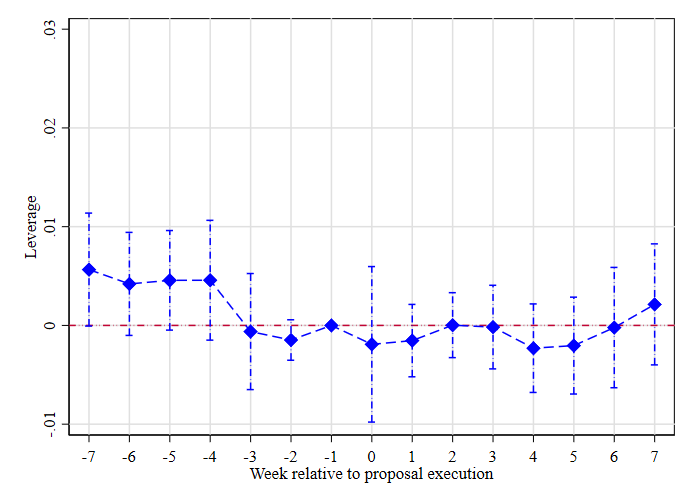
\includegraphics[width=0.45\linewidth]{figure/Heterogeneity/lev_g1.png}}
\subfloat[Quartile 2]{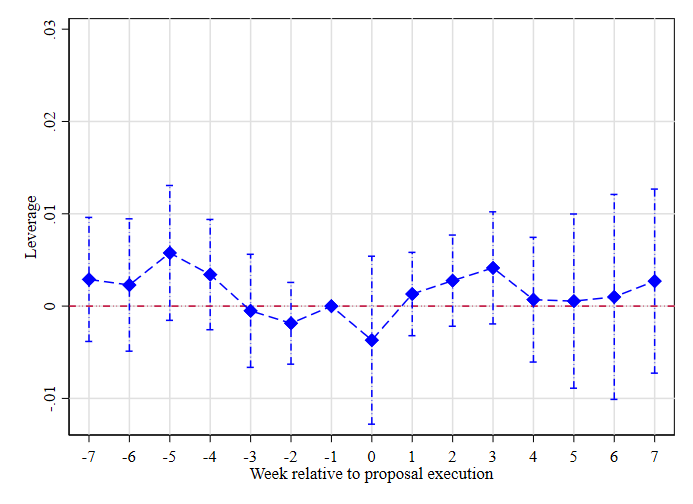
\includegraphics[width=0.45\linewidth]{figure/Heterogeneity/lev_g2.png}}

\subfloat[Quartile 3]{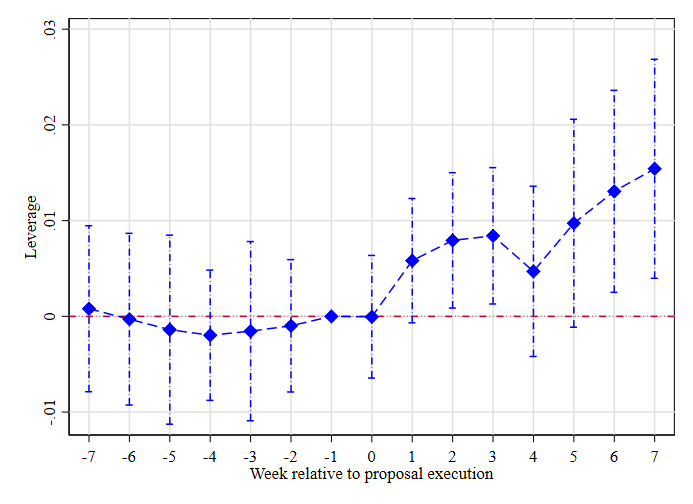
\includegraphics[width=0.45\linewidth]{figure/Heterogeneity/lev_g3.png}}
\subfloat[Quartile 4 (Highest Leverage)]{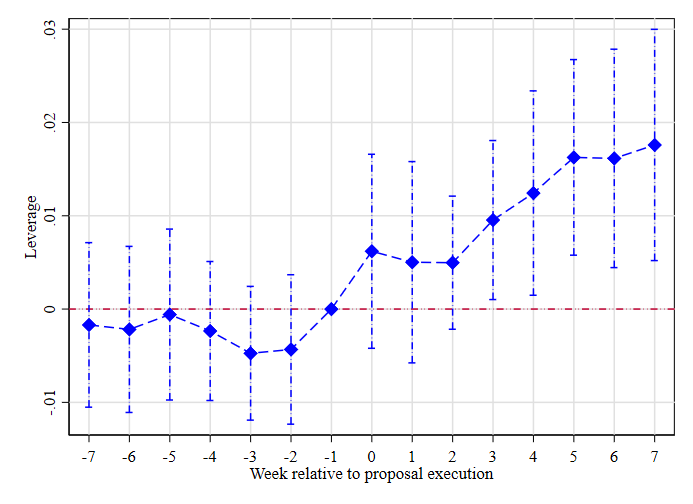
\includegraphics[width=0.45\linewidth]{figure/Heterogeneity/lev_g4.png}}

\end{figure}

\end{landscape}


\clearpage
\newpage



% \begin{landscape}
\begin{figure}[ht!]
\centering
\caption{Dynamics of Interest Rates of Stablecoins}\label{fig:dynamics_interestrates}
\caption*{This figure plots the estimations of $\beta$ coefficients from the OLS regression: $ Y_{c,t}^p=\sum_{j=-7}^{7}\beta_jTreated_{c}^p\times I_j+\delta Treated_{c}^p+\sum_{s=-7}^{7}\sigma_sI_s+ \textit{Crypto}\times\textit{Week FE}+\epsilon_{c,t}^p$, where $Y_{c,t}^p$ represents one of the utilization ratios, lending rates, and borrowing rates of cryptocurrency $c$ on platform $p$ at the end of week $t$. $Treated_{c}^{p}$ is a binary variable that takes a value of 1 if platform $p$, operating the cryptocurrency pool $c$, relaxes the margin requirements. $I_j$ is an indicator variable for weeks relative to the week of proposal execution. Standard errors are clustered at week levels. The bars surrounding each coefficient represent the 5\% and 95\% confidence intervals. }

\bigskip

% \subfloat[Deposit (Dollar)]{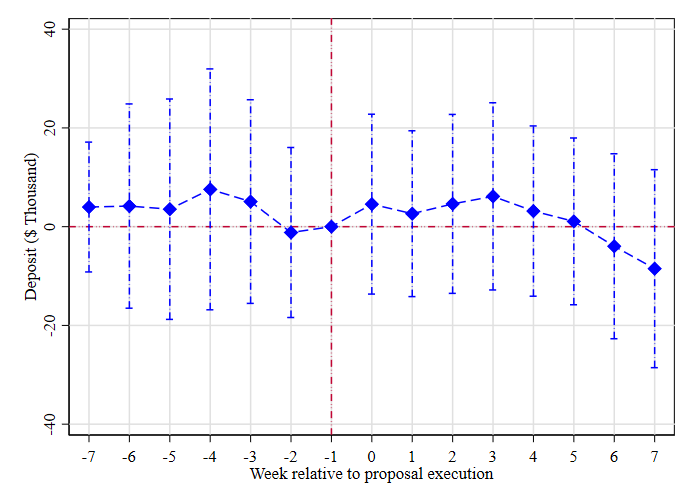
\includegraphics[width=0.45\linewidth]{figure/deposit_dollar.png}}
\subfloat[Utilization Ratio]{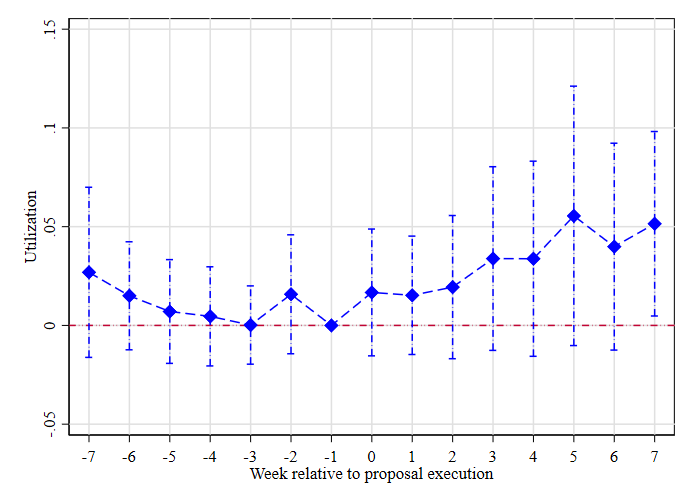
\includegraphics[width=\linewidth]{figure/Utilization.png}}

\end{figure}

% \end{landscape}

\clearpage
\newpage
\begin{figure}[ht!]
\ContinuedFloat 

\centering
\caption*{ Figure \ref{fig:dynamics_interestrates} - Continued from the previous page}
\subfloat[Lending Rate (\%)]{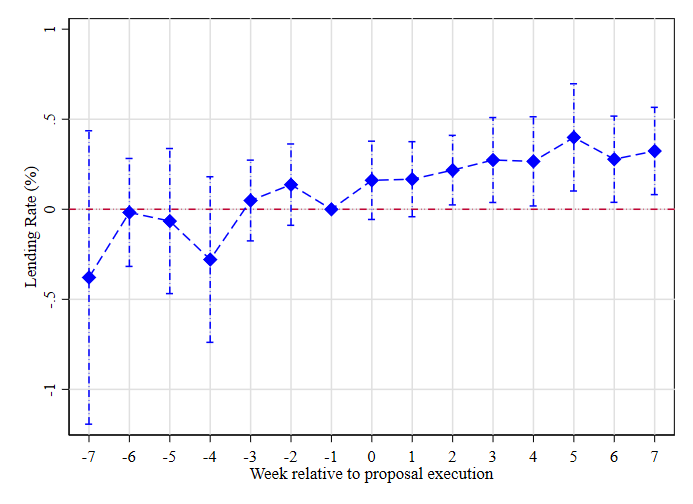
\includegraphics[width=0.85\linewidth]{figure/LendingRate.png}}

\subfloat[Borrowing Rate (\%)]{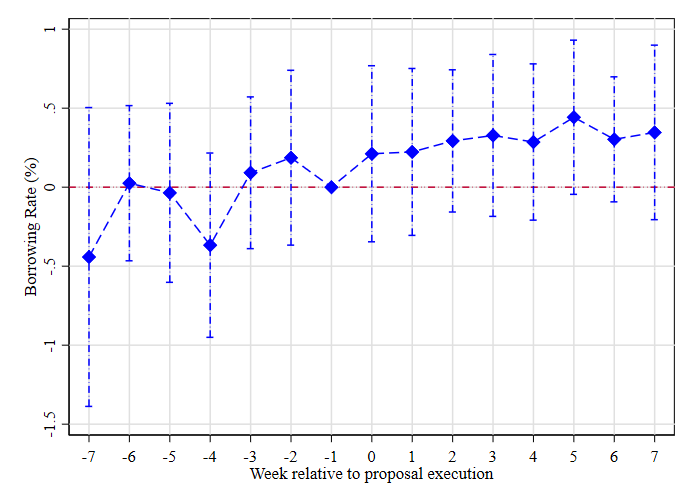
\includegraphics[width=0.85\linewidth]{figure/BorrowingRate.png}}

\end{figure}

